%%=============================================================================
%% Methodologie
%%=============================================================================

\chapter{\IfLanguageName{dutch}{Hoe kan het beter?}{Results}}%
\label{ch:beter}



\section{Literatuuroverzicht}

In aanvulling op de eerder besproken stand van zaken biedt dit literatuuroverzicht een verdiepend inzicht in het gebruik van Mendix als low-code platform op basis van bestaande literatuur, praktijkcases en academisch onderzoek. Het platform, dat bekend staat om zijn visuele ontwikkelomgeving en ondersteuning voor zowel professionele als niet-technische gebruikers, wordt steeds vaker ingezet voor snelle en iteratieve applicatieontwikkeling \autocite{Alamin2021}. Daarnaast zijn er diverse praktijkvoorbeelden en academische analyses die de voordelen en beperkingen van low-code ontwikkeling, en Mendix in het bijzonder, verder belichten \autocite{Gadia2025}.
\subsection{Praktijkvoorbeelden en Casestudies}
Diverse organisaties hebben Mendix succesvol ingezet voor uiteenlopende toepassingen:
\begin{itemize}
    \item \textbf{Gemeente Rotterdam}
    \\
    Door het gebruik van Mendix heeft de gemeente meer dan 100 low-code applicaties ontwikkeld, waaronder een COVID-responsportaal en een parkeervergunning-app. Deze applicaties ondersteunen meer dan 100.000 gebruikers en zijn gemiddeld binnen 8-12 weken ontwikkeld \autocite{Mendix2025a}.
    \item \textbf{PostNL}
    \\
    Het nationale postbedrijf van Nederland heeft zijn ordermanagementsysteem herbouwd met Mendix, gebruikmakend van een microservices-architectuur. Hierdoor kunnen ze meer dan 1 miljoen pakketten per dag verwerken en hebben ze een achterstand van twee jaar in zes maanden weggewerkt \autocite{Zaman2024}.
    \item \textbf{AZL}
    \\
    Deze pensioenfondsbeheerder heeft met Mendix een klantportaal ontwikkeld dat het pensioenkeuzeproces voor deelnemers vereenvoudigt. Door de overstap naar een agile werkwijze in combinatie met low-code ontwikkeling, konden ze sneller inspelen op klantbehoeften en de gebruikerservaring verbeteren \autocite{MendixAZL}.
\end{itemize}
\subsection{Ervaringen en Knelpunten uit Ontwikkelaarsgemeenschappen}
Onderzoek naar discussies op platforms zoals Stack Overflow en Reddit onthult dat ontwikkelaars verschillende uitdagingen ervaren bij het gebruik van low-code platforms:
\begin{itemize}
    \item \textbf{Aanpassingsmogelijkheden}
    \\
    Veel ontwikkelaars ondervinden moeilijkheden bij het aanpassen van gebruikersinterfaces en het implementeren van dynamische event-handling in low-code omgevingen. Een studie toonde aan dat meer dan 40\% van de vragen op Stack Overflow betrekking had op dergelijke aanpassingen, waarbij een significant deel onbeantwoord bleef \autocite{Alamin2021}.
    \item \textbf{Integratie met externe systemen}
    \\
    Hoewel platforms als Mendix en OutSystems integratiemogelijkheden bieden, ervaren ontwikkelaars soms beperkingen bij het koppelen van specifieke externe systemen of bij het beheren van complexe dataflows \autocite{Gadia2025}.
\end{itemize}
\subsection{Academische Inzichten in Low-Code Ontwikkeling}
Academisch onderzoek benadrukt zowel de voordelen als de uitdagingen van low-code ontwikkeling:
\begin{itemize}
    \item \textbf{Versnelling van ontwikkelprocessen}
    \\
    Low-code platforms stellen organisaties in staat om sneller applicaties te ontwikkelen, wat met name voordelig is in domeinen die behoefte hebben aan geautomatiseerde processen en workflows \autocite{Luo2021}.
    \item \textbf{Beperkingen in complexiteit}
    \\
    Hoewel low-code geschikt is voor veel toepassingen, kunnen er beperkingen zijn bij het ontwikkelen van zeer complexe of gespecialiseerde applicaties, waarbij traditionele programmeertalen meer flexibiliteit bieden.
\end{itemize}







\section{Praktisch onderzoek}
In dit praktisch onderzoek worden twee applicaties met elkaar vergeleken: één ontwikkeld met het low-code platform Mendix en één ontwikkeld met JavaScript en React. 

\begin{figure}[H]
    \centering
    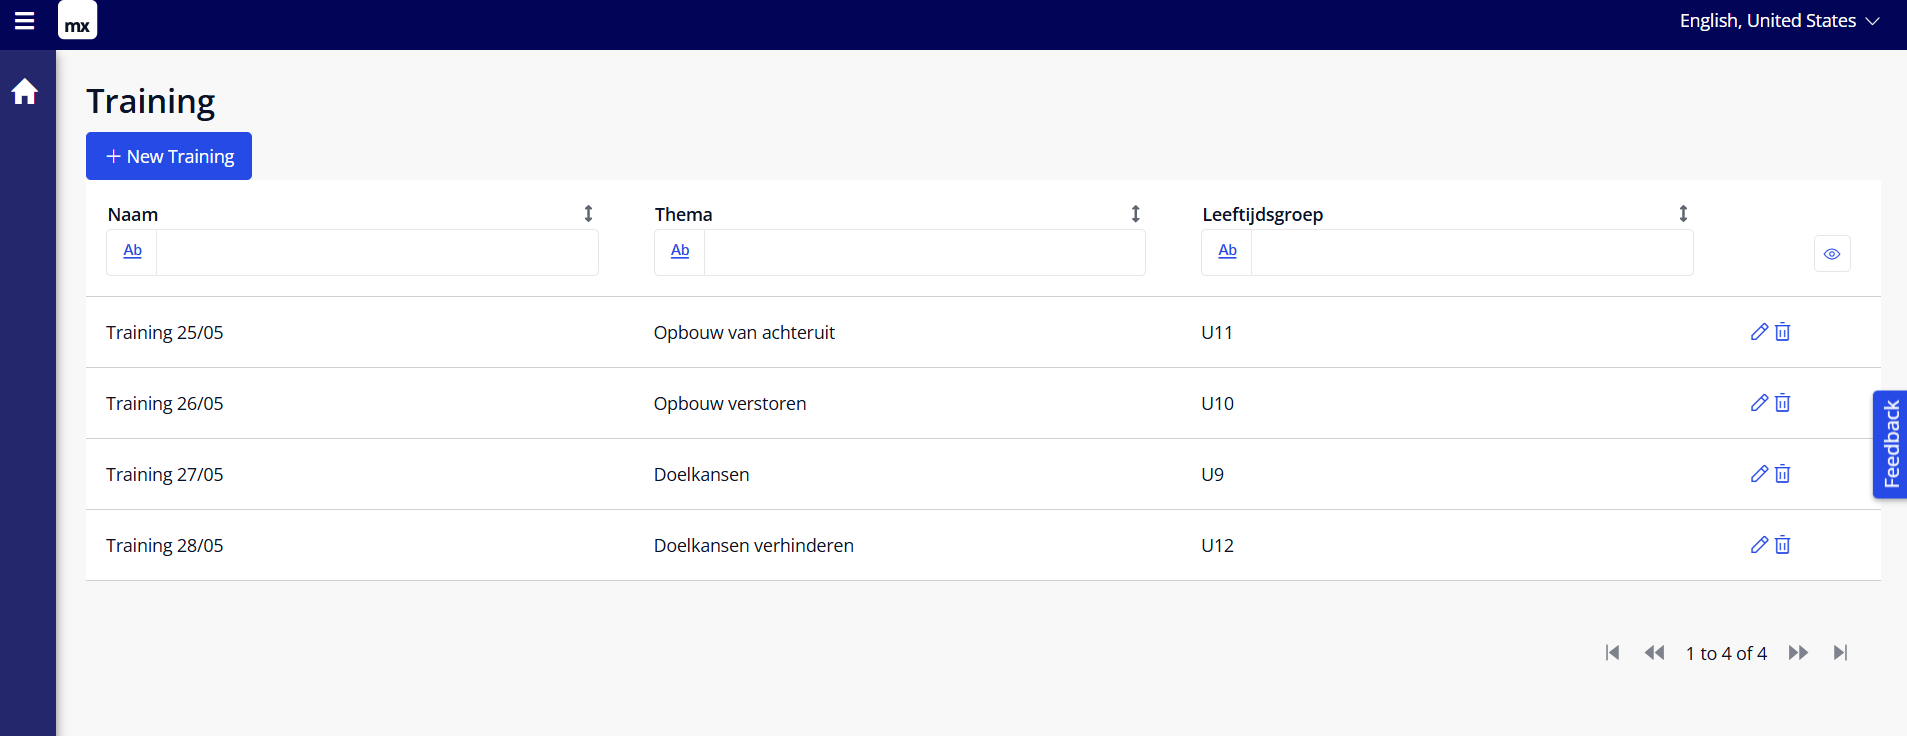
\includegraphics[width=0.8\textwidth]{Homepage-Mendix.png}
    \caption[Homepage Mendix applicatie]{\label{fig:homepage-mendix} Homepage Mendix applicatie }
\end{figure}

\begin{figure}[H]
    \centering
    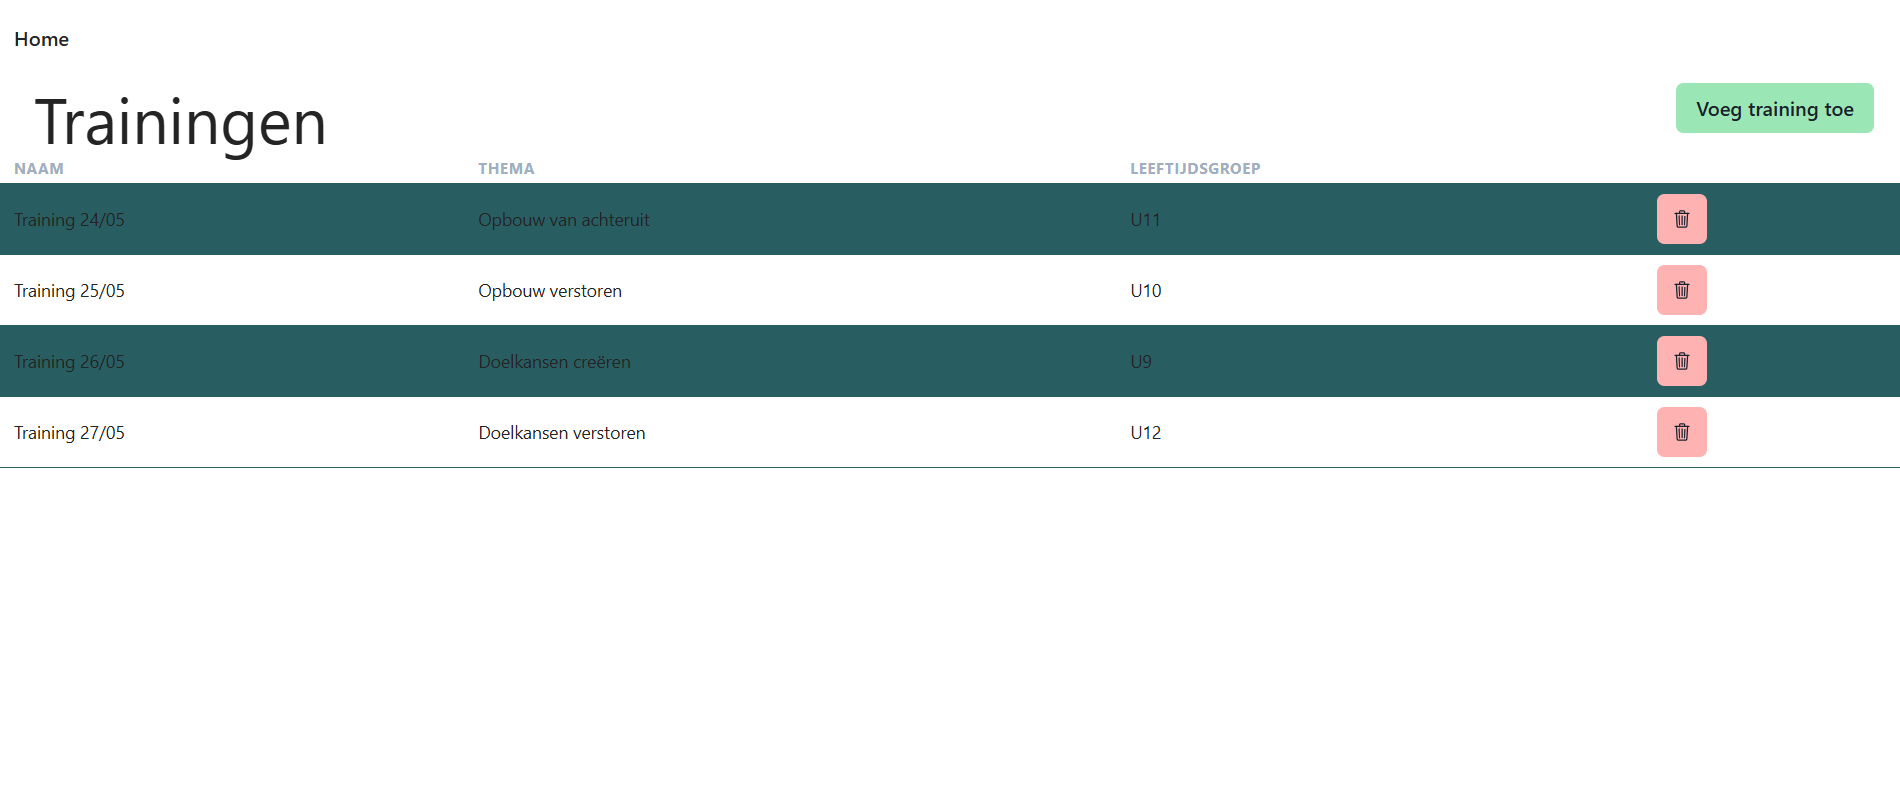
\includegraphics[width=0.8\textwidth]{Homepage-JS.png}
    \caption[Homepage Mendix applicatie]{\label{fig:homepage-JavaScript} Homepage JavaScript/React applicatie }
\end{figure}

Het doel van deze vergelijking is om inzicht te krijgen in de sterktes en beperkingen van beide technologieën op basis van praktijkgerichte criteria. De evaluatie richt zich op zes hoofdgebieden: prestatie en schaalbaarheid, integratiemogelijkheden, aanpasbaarheid en uitbreidbaarheid, ontwikkelsnelheid, beveiliging en compliance, en de algehele gebruikerservaring. Voor elk van deze categorieën worden gerichte testen uitgevoerd, variërend van technische benchmarks (zoals laadtijd en load testing) tot ontwikkelervaring en gebruiksvriendelijkheid. Door beide applicaties op systematische wijze te testen, wordt duidelijk in welke scenario’s Mendix of juist een traditionele JavaScript/React-stack de voorkeur verdient. De resultaten uit deze vergelijking vormen de basis voor de uiteindelijke conclusie over de toepasbaarheid van beide benaderingen binnen diverse zakelijke contexten.
\subsection{Schaalbaarheid en prestaties}
Om een objectieve vergelijking te kunnen maken tussen de in Mendix en in JavaScript/React ontwikkelde applicaties, zijn verschillende prestatie- en schaalbaarheidstesten uitgevoerd. Deze testen richten zich op drie kernaspecten: de laadtijd van de applicatie, de reactietijd op gebruikersacties en de prestaties onder belasting. Voor het meten van de laadtijd zijn tools zoals Google Lighthouse en Chrome DevTools gebruikt, waarmee onder andere de \gls{FCP} en de \gls{LCP} zijn geanalyseerd. Daarnaast is de reactietijd op interacties met de gebruikersinterface gemeten om de responsiviteit van beide applicaties te beoordelen. Tot slot wordt een load test uitgevoerd met tools als Apache JMeter en k6 om inzicht te krijgen in de schaalbaarheid en het gedrag van de applicaties bij een hoge gebruikersbelasting. Deze metingen geven een duidelijk beeld van de praktische prestaties van beide technologieën in een realistische gebruiksomgeving.

\subsubsection{Laadtijd (Performance)}
De laadtijd van een webapplicatie is een cruciale factor voor de gebruikerservaring, aangezien gebruikers doorgaans verwachten dat een pagina binnen 2 à 3 seconden volledig geladen is. Om de prestaties van beide applicaties objectief te meten, werd gebruikgemaakt van Google Lighthouse. Deze tool analyseert verschillende web performance-indicatoren, waaronder:
\begin{itemize}
    \item \gls{FCP}
    \item \gls{LCP}
    \item \gls{TBT}
    \item Speed Index
    \item \gls{CLS}
    \item Performance Score (algemene score op 100)
\end{itemize}

\subsubsection{Resultaten}

Voor zowel de Mendix-applicatie als de JavaScript/React-applicatie werden telkens drie afzonderlijke metingen uitgevoerd. De resultaten van deze testen zijn gemiddeld om zo een eerlijke vergelijking te maken. In onderstaande tabel worden de gemiddelde waarden van de prestaties per platform weergegeven, inclusief een kolom met het rekenkundig gemiddelde tussen de twee platformen ter referentie.

\newpage
\paragraph{JavaScript/React resultaten laadtijd}

\begin{table}[h]
    \centering
    \begin{tabular}{ |p{3cm}|p{2.75cm}|p{2.75cm}|p{2.75cm}|p{2.75cm}|}
        \hline
        \textbf{Metriek} & \textbf{Test 1} & \textbf{Test 2}  & \textbf{Test 3} & \textbf{Gemiddelde}\\
        \hline
        \textbf{\gls{FCP}}  & 11.8s & 11.8s & 11.7s & 11.8s \\
        \hline
        \textbf{\gls{LCP}} & 22.8s & 22.9s & 22.6s & 22.8s\\
        \hline
        \textbf{\gls{TBT}}  & 540ms & 610ms & 340ms & 497ms \\
        \hline
        \textbf{Speed Index}  & 11.8s & 11.8s & 11.7s & 11.8s \\
        \hline
        \textbf{\gls{CLS}}  & 0 & 0  & 0 & 0 \\
        \hline
        \textbf{Performance Score}  & 42 & 40  & 48 & 43 \\
        \hline
    \end{tabular}
    \caption[\centering Testresultaten laadtijd JavaScript/React]{\label{tab:Testresultaten JavaScript/React}Testresultaten JavaScript/React.}
\end{table}

\begin{figure}[htbp]
    \centering
    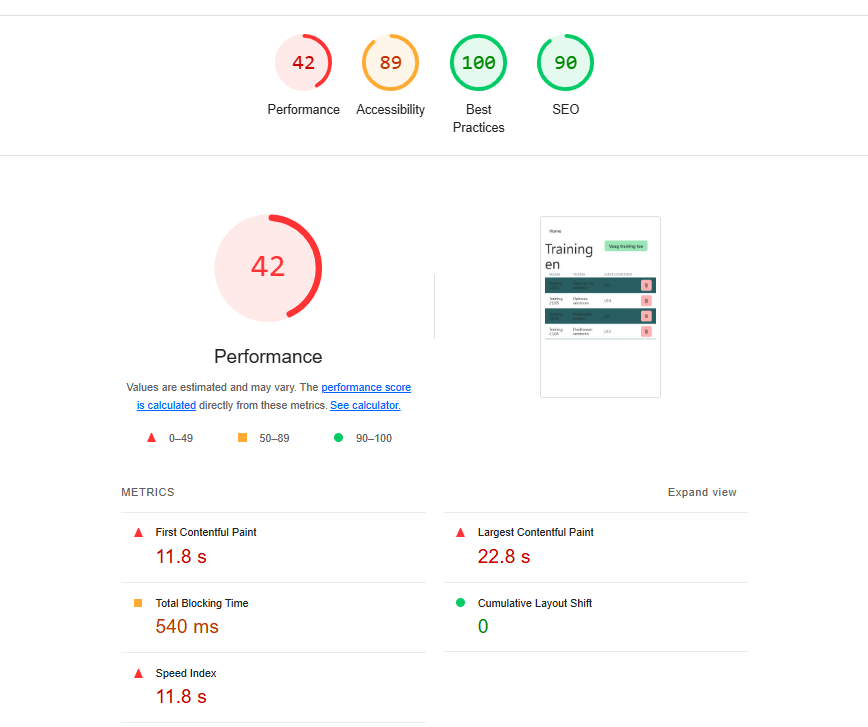
\includegraphics[width=0.3\textwidth]{JS-test1.png}
    \hfill
    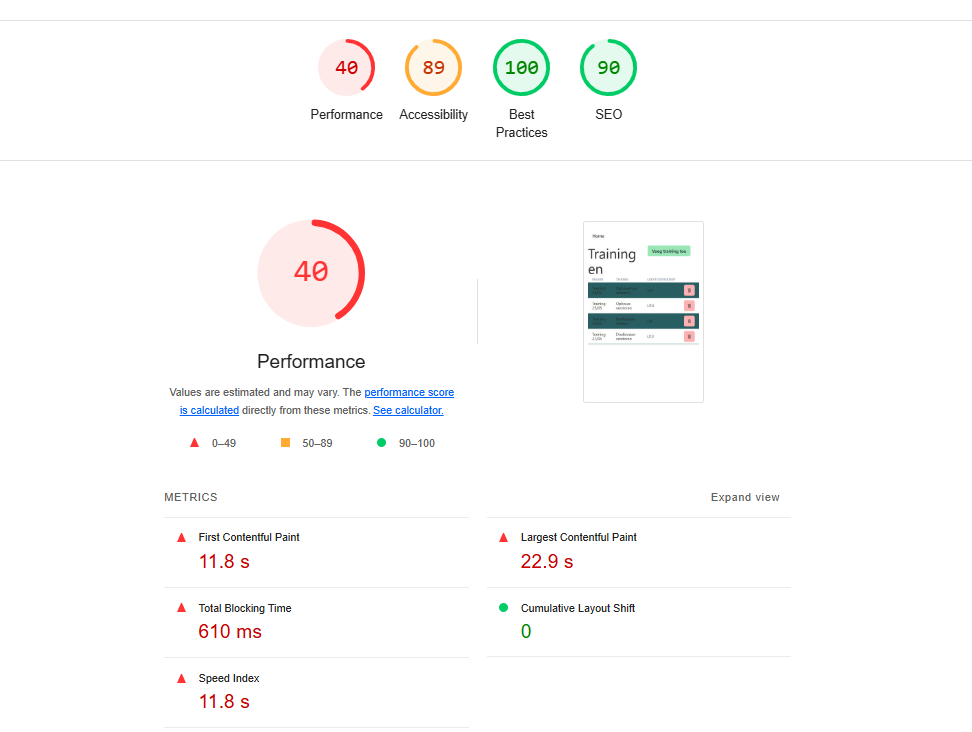
\includegraphics[width=0.3\textwidth]{JS-test2.png}
    \hfill
    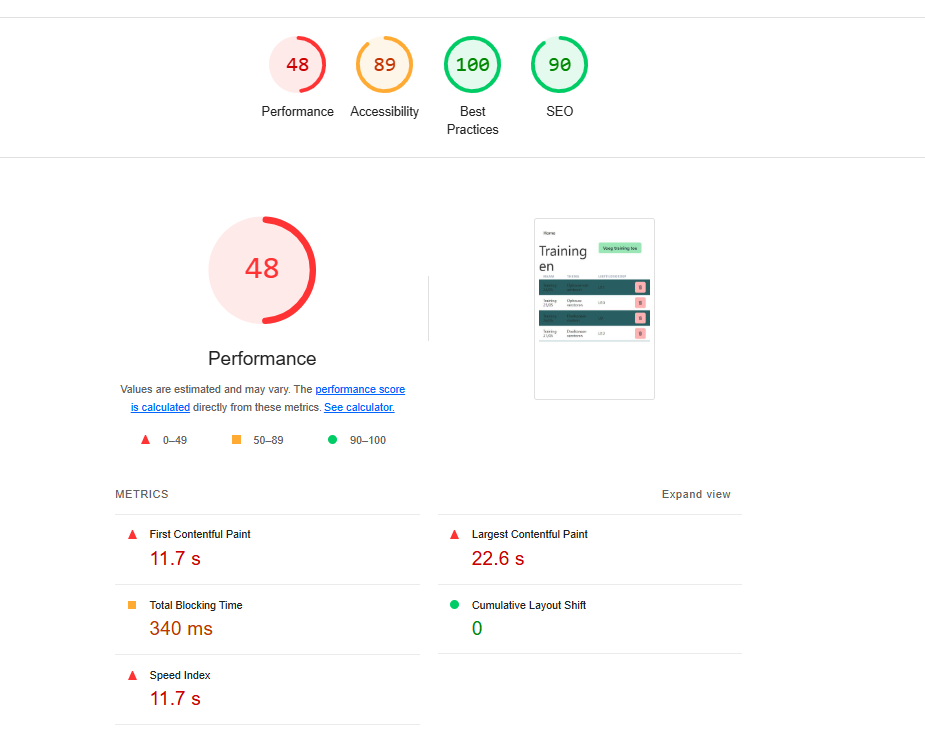
\includegraphics[width=0.3\textwidth]{JS-test3.png}
    \caption{Lighthouse testresultaten JavaScript/React - Links: Test 1, Midden: Test 2, Rechts: Test 3}
    \label{fig:javascript-simple}
\end{figure}

\newpage
\paragraph{Mendix resultaten laadtijd}

\begin{table}[h]
    \centering
    \begin{tabular}{ |p{3cm}|p{2.75cm}|p{2.75cm}|p{2.75cm}|p{2.75cm}|}
        \hline
        \textbf{Metriek} & \textbf{Test 1} & \textbf{Test 2}  & \textbf{Test 3} & \textbf{Gemiddelde}\\
        \hline
        \textbf{\gls{FCP}}  & 13.7s & 13.9s & 13.7s & 13.8s \\
        \hline
        \textbf{\gls{LCP}} & 17.8s & 18.2s & 17.8s & 17.9s\\
        \hline
        \textbf{\gls{TBT}}  & 330ms & 500ms & 260ms & 363ms \\
        \hline
        \textbf{Speed Index}  & 13.7s & 13.9s & 13.7s & 13.8s \\
        \hline
        \textbf{\gls{CLS}}  & 0 & 0  & 0 & 0 \\
        \hline
        \textbf{Performance Score}  & 48 & 43  & 50 & 47 \\
        \hline
    \end{tabular}
    \caption[\centering Testresultaten laadtijd Mendix]{\label{tab:Testresultaten Mendix}Testresultaten Mendix}
\end{table}

\begin{figure}[htbp]
    \centering
    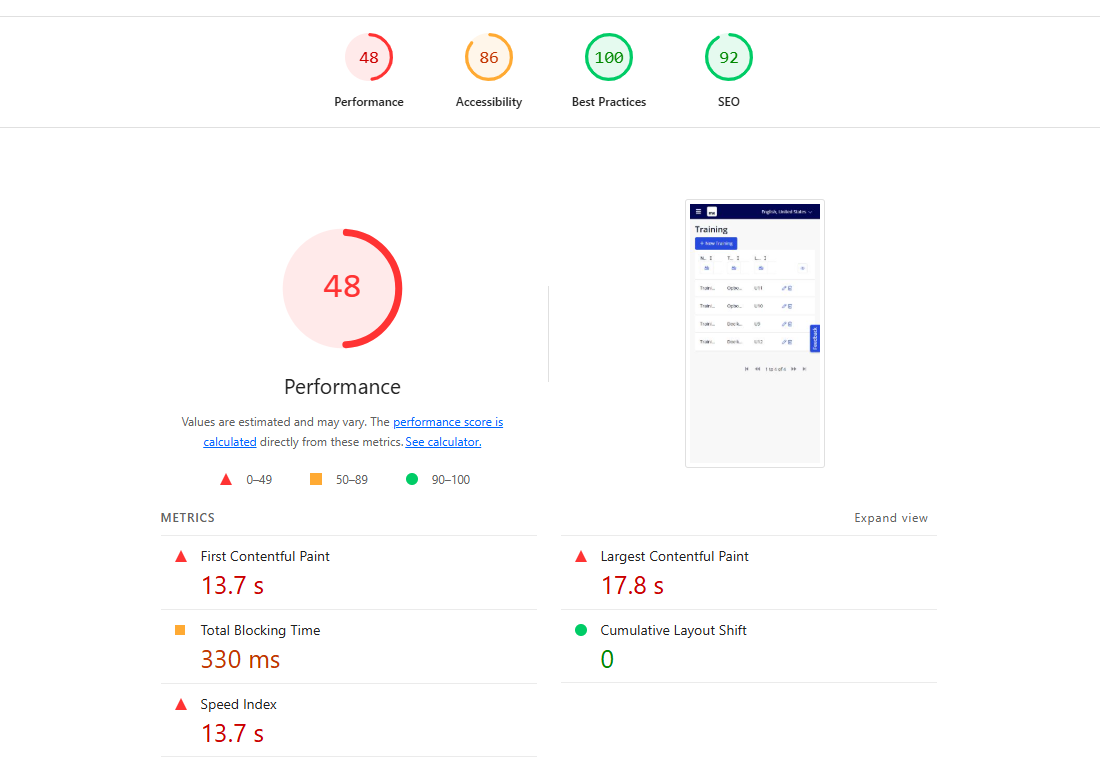
\includegraphics[width=0.3\textwidth]{Mendix-test1.png}
    \hfill
    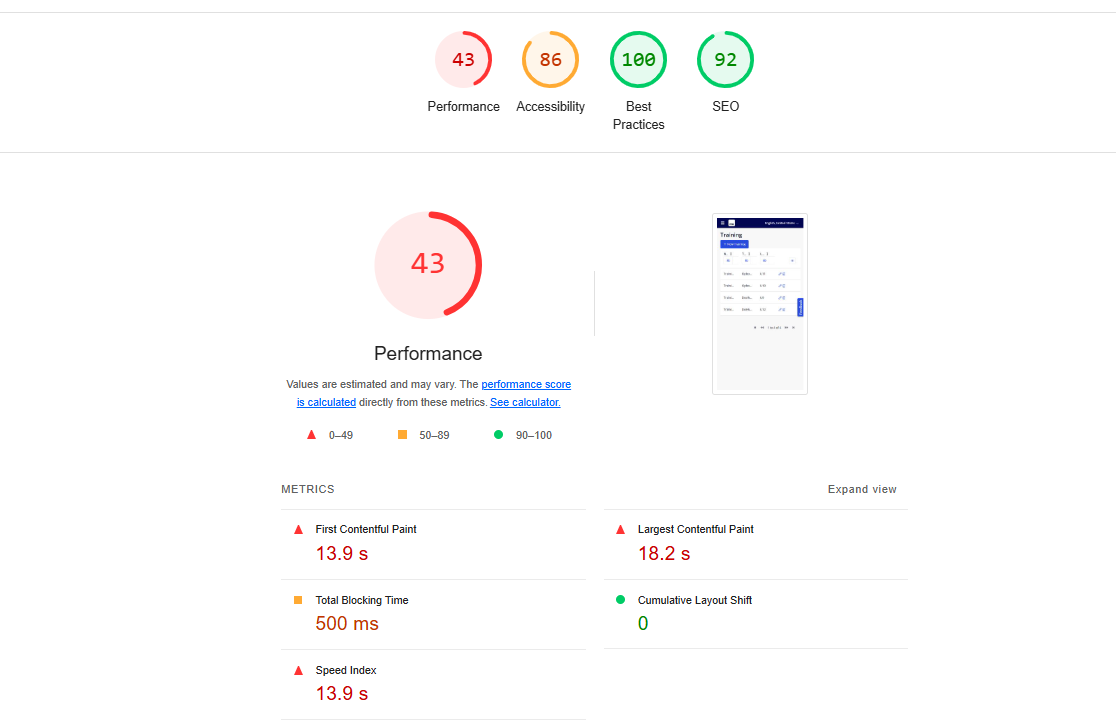
\includegraphics[width=0.3\textwidth]{Mendix-test2.png}
    \hfill
    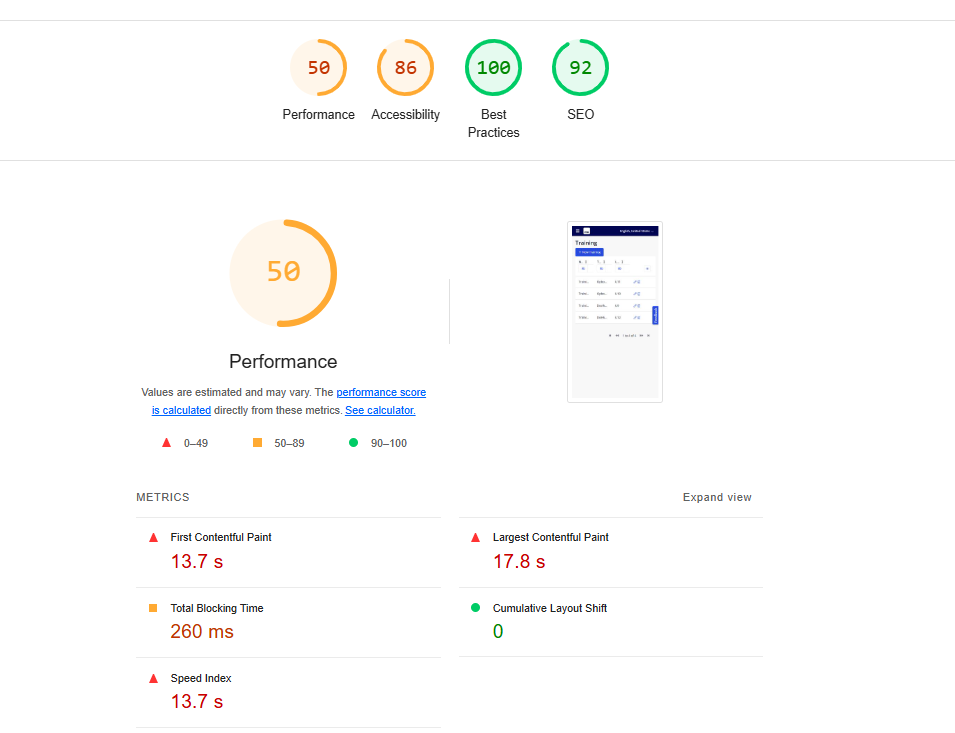
\includegraphics[width=0.3\textwidth]{Mendix-test3.png}
    \caption{Lighthouse testresultaten Mendix - Links: Test 1, Midden: Test 2, Rechts: Test 3}
    \label{fig:mendix-simple}
\end{figure}
\newpage
\paragraph{Vergelijkingstabel}
\begin{table}[h]
    \centering
    \begin{tabular}{ |p{3cm}|p{2.25cm}|p{2.25cm}|p{2.25cm}|p{3.25cm}|}
        \hline
        \textbf{Metriek} & \textbf{JavaScript/} \newline \textbf{React} & \textbf{Mendix}  & \textbf{Verschil} & \textbf{Beste Prestatie}\\
        \hline
        \textbf{\gls{FCP}}  & 11.8s & 13.8s & -2.0s & JavaScript/React \\
        \hline
        \textbf{\gls{LCP}} & 22.8s & 17.8s & +4.9s & Mendix\\
        \hline
        \textbf{\gls{TBT}}  & 497msms & 363ms & +134ms & Mendix \\
        \hline
        \textbf{Speed Index}  & 11.8s & 13.8s & -2.0s & JavaScript/React \\
        \hline
        \textbf{\gls{CLS}}  & 0 & 0  & Gelijk & Gelijk \\
        \hline
        \textbf{Performance Score}  & 43 & 47  & -4 & Mendix \\
        \hline
    \end{tabular}
    \caption[\centering Vergelijkingstabel laadtijd]{\label{tab:Vergelijkingstabel laadtijd}Vergelijkingstabel laadtijd}
\end{table}

\paragraph{Samenvatting}
\begin{itemize}
    \item JavaScript/React is sneller bij \gls{FCP} en Speed Index (2s sneller)
    \item Mendix presteert beter bij \gls{LCP} (4,9s sneller) en \gls{TBT} (134ms minder)
    \item Mendix heeft een hogere Performance Score (47 vs 43)
    \item Beide platforms hebben perfecte \gls{CLS} scores
    \item Beide platforms scoren onder acceptabele performance niveaus (<50)
\end{itemize}
De prestatieverschillen tussen Mendix en JavaScript/React kunnen verklaard worden door fundamentele verschillen in architectuur en uitvoering. JavaScript/React scoort beter op \gls{FCP} doordat het doorgaans gebruikmaakt van een lichte initiële bundel en client-side rendering, waardoor visuele elementen snel zichtbaar zijn. Mendix presteert daarentegen beter op \gls{LCP} en \gls{TBT} dankzij de geïntegreerde backend, geoptimaliseerde dataverwerking en beperkte client-side JavaScript. Door logica server-side af te handelen en automatisch platformoptimalisaties toe te passen, vermindert Mendix de belasting op de browser, wat resulteert in betere prestaties bij het laden van grote elementen en minder blokkeringen tijdens interacties.

\subsubsection{Reactietijd op gebruikersacties}
De reactietijd van een webapplicatie, oftewel de tijd tussen een gebruikersactie (zoals een klik) en het zichtbare resultaat , is essentieel voor een vloeiende gebruikerservaring. Gebruikers verwachten dat interacties vrijwel onmiddellijk reageren, idealiter binnen 100 tot 200 milliseconden. Om de reactietijd objectief te evalueren, werd een handmatige performance-analyse uitgevoerd met behulp van de ontwikkelaarstools in Google Chrome (Performance tab). 

\subsubsection{Resultaten}
Bij de testen werd specifiek gekeken naar het toevoegen van een nieuw item binnen zowel de Mendix- als de JavaScript/React-applicatie. Door de belangrijkste fasen van dit proces in kaart te brengen, van het moment waarop een gebruiker een actie uitvoert tot aan de visuele terugkoppeling op het scherm, kon een nauwkeurige vergelijking worden gemaakt van de snelheid en efficiëntie van beide implementaties.

\paragraph{JavaScript/React resultaten reactietijd}

\begin{figure}[H]
    \centering
    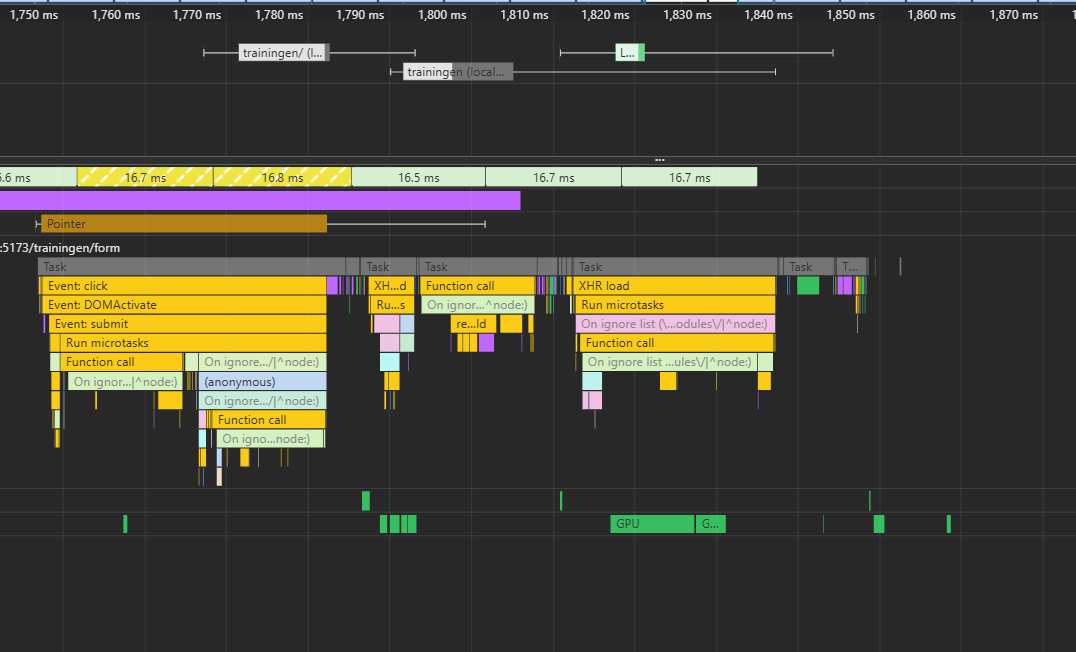
\includegraphics[width=0.8\textwidth]{Test JS reactietijd Toevoegen.png}
    \caption[Testresultaten toevoegen object in JavaScript/React]{\label{fig:reactietijd-JavaScript} Testresultaten toevoegen object in JavaScript/React }
\end{figure}


\begin{table}[H]
    \centering
    \begin{tabular}{ |p{5cm}|p{3cm}|p{6cm}|}
        \hline
        \textbf{Metriek} & \textbf{Tijd/Duur} & \textbf{Beschrijving}\\
        \hline
        \textbf{Start operatie/ Event Click}  & $\sim$1.750 ms & Start van gebruikersinteractie \\
        \hline
        \textbf{\gls{DOM} Activate} & $\sim$1.752 ms & Verwerking van DOM-event \\
        \hline
        \textbf{Event Submit}  & $\sim$1.754 ms & Formulier wordt verstuurd \\
        \hline
        \textbf{Microtasks}  & 1.754 – 1.756 ms & Uitvoering van JavaScript-taken \\
        \hline                       
        \textbf{\gls{XHR} Load}  & 1.790 – 1.820 ms & Communicatie met de server  \\
        \hline
        \textbf{Function Calls}  & 1.820 – 1.840 ms & Verwerking van de serverrespons \\
        \hline
        \textbf{GPU Rendering}  & $\sim$1.850 ms & 	Visuele weergave (rendering) \\
        \hline
        \textbf{Reactietijd}  & ≈ 100 ms & 	Tijdsduur van klik tot weergave \\
        \hline
    \end{tabular}
    \caption[\centering Testresultaten reactietijd JavaScript/React]{\label{tab:Testresultaten JS reactietijd}Testresultaten reactietijd JavaScript/React}
\end{table}

\begin{table}[H]
    \centering
    \begin{tabular}{ |p{5cm}|p{3cm}|p{6cm}|}
        \hline
        \textbf{Fase} & \textbf{Duur} & \textbf{Activiteit}\\
        \hline
        \textbf{Eventverwerking}  & $\sim$4 ms & Van klik tot submit \\
        \hline
        \textbf{\gls{XHR}-verzoek} & $\sim$30 ms & Verzoek naar en antwoord van de server \\
        \hline
        \textbf{Responsverwerking}  & $\sim$20 ms & Verwerking van ontvangen data \\
        \hline
        \textbf{Visuele rendering}  & $\sim$46 ms & \gls{UI} wordt bijgewerkt op het scherm \\
        \hline                       

    \end{tabular}
    \caption[\centering Breakdown reactietijd JavaScript/React]{\label{tab:breakdown JS reactietijd}Breakdown reactietijd JavaScript/React}
\end{table}



\newpage




\paragraph{Mendix resultaten reactietijd}

\begin{figure}[H]
    \centering
    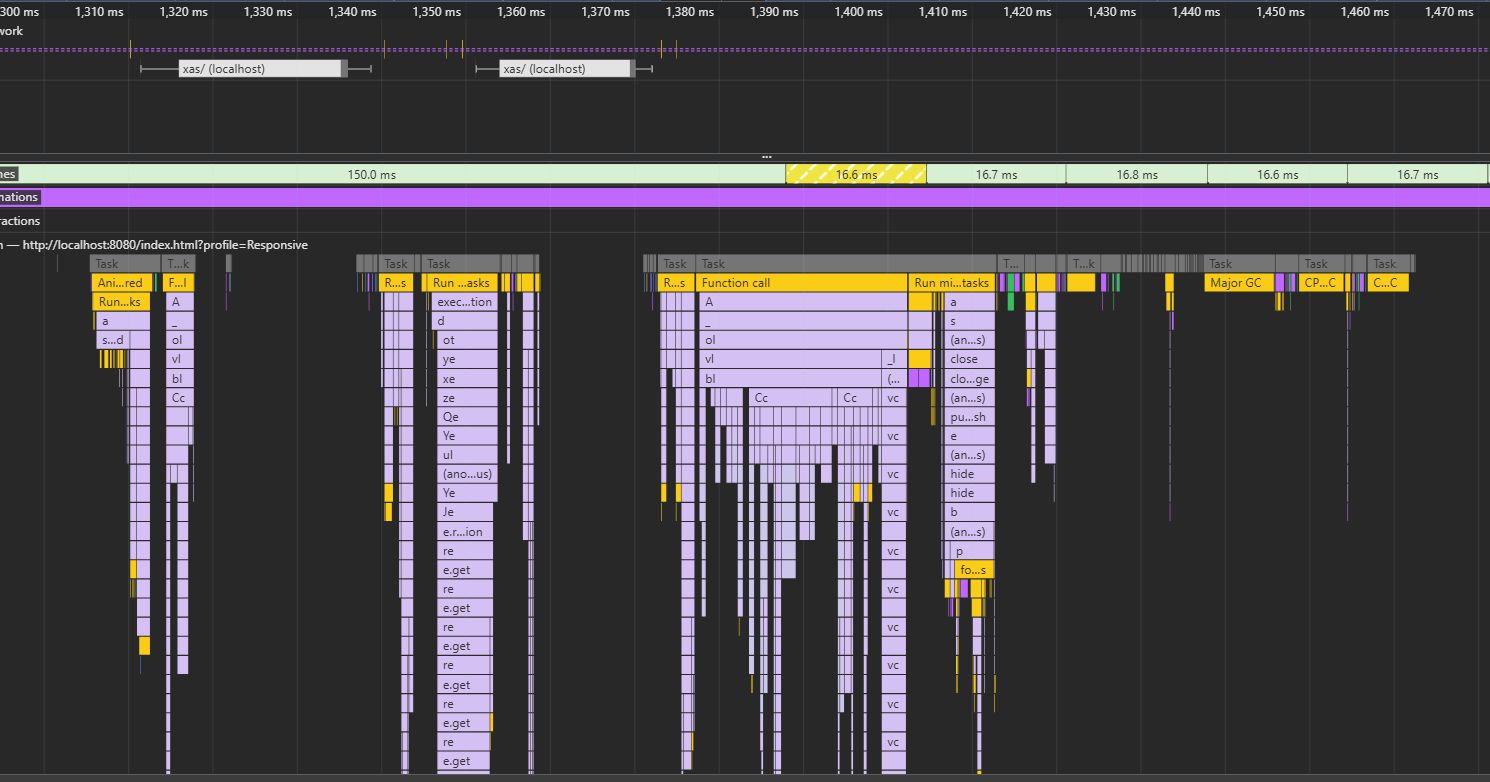
\includegraphics[width=0.8\textwidth]{Test Mendix reactietijd Toevoegen.png}
    \caption[Testresultaten toevoegen object in Mendix]{\label{fig:reactietijd-Mendix} Testresultaten toevoegen object in Mendix}
\end{figure}


\begin{table}[h]
    \centering
    \begin{tabular}{ |p{5cm}|p{3cm}|p{6cm}|}
        \hline
        \textbf{Metriek} & \textbf{Tijd/Duur} & \textbf{Beschrijving}\\
        \hline
        \textbf{Start operatie}  & $\sim$1.300 ms & Start van gebruikersinteractie \\
        \hline
        \textbf{Animation/Render} & 1.300 - 1.320 ms & \gls{UI} animaties en rendering \\
        \hline
        \textbf{Run Tasks}  & 1.320 - 1.340 ms & Asynchrone task verwerking \\
        \hline
        \textbf{Function Calls}  & 1.340 - 1.380 ms & Core applicatie logica \\
        \hline                       
        \textbf{Major \gls{GC}}  & 1.790 – 1.820 ms & Communicatie met de server  \\
        \hline
        \textbf{Function Calls}  & 	$\sim$1.440 ms & Garbage collection \\
        \hline
        \textbf{Operatie Compleet}  & $\sim$1.470 ms & 	Item volledig toegevoegd \\
        \hline
        \textbf{Totale reactietijd}  & ≈ 170 ms & Tijdsduur van klik tot weergave \\
        \hline
    \end{tabular}
    \caption[\centering Testresultaten reactietijd Mendix]{\label{tab:Testresultaten Mendix reactietijd}Testresultaten reactietijd Mendix}
\end{table}

\begin{table}[H]
    \centering
    \begin{tabular}{ |p{5cm}|p{3cm}|p{6cm}|}
        \hline
        \textbf{Fase} & \textbf{Duur} & \textbf{Activiteit}\\
        \hline
        \textbf{Initial Animation}  & $\sim$20 ms & \gls{UI} feedback start \\
        \hline
        \textbf{Task Processing} & $\sim$20 ms & Asynchrone verwerking \\
        \hline
        \textbf{Function Execution}  & $\sim$40 ms & Business logica \\
        \hline
        \textbf{Rendering and \gls{GC}}  & $\sim$90 ms & \gls{UI} updates + cleanup \\
        \hline                       
        
    \end{tabular}
    \caption[\centering Breakdown reactietijd Mendix]{\label{tab:breakdown Mendix reactietijd}Breakdown reactietijd Mendix}
\end{table}


\pagebreak
\newpage


\paragraph{Conclusie}
Hoewel JavaScript met 100 ms iets sneller is dan Mendix met 170 ms van start tot completion, is het verschil van 70 ms relatief klein en valt het binnen een categorie van zeer responsieve prestaties. JavaScript profiteert van snellere verwerking, maar omvat ook een server roundtrip van ongeveer 30 ms via \gls{XHR} calls, terwijl Mendix juist meer lokale verwerking en garbage collection uitvoert, wat zorgt voor extra framework overhead. Beide platformen tonen vergelijkbare tijden voor de kernlogica (~50-60 ms), wat aangeeft dat het verschil vooral zit in de UI rendering en framework processing. Voor een kleine applicatie is deze lichte vertraging in Mendix een acceptabele trade-off, gezien de rijkere functionaliteit en gebruikerservaring die het biedt. Bij grotere en complexere applicaties kan de Mendix overhead echter toenemen, wat de prestaties meer beïnvloedt. Desondanks leveren beide technologieën een vrijwel directe respons die gebruikers als “instant” ervaren, waardoor deze realistische vergelijking een eerlijk beeld geeft van de praktische prestaties in echte toepassingen.



\subsubsection{Load test}
Om de schaalbaarheid en robuustheid van de webapplicaties te evalueren onder verschillende belastingniveaus, werden ook loadtesten uitgevoerd. Deze testen simuleren een toenemend aantal gelijktijdige gebruikers om te bepalen hoe de applicaties presteren onder stress en om eventuele knelpunten te identificeren.

\subsubsection{Resultaten}
De loadtesten zijn uitgevoerd door het simuleren van HTTP-verzoeken voor een oplopend aantal gebruikers (10, 100, 250, 500, 1000, 2500 gebruikers) voor zowel de Mendix- als de JavaScript/React-applicatie. Hierbij is gebruikgemaakt van Apache JMeter, een veelgebruikte tool voor het uitvoeren van prestatietests, waarmee realistische gebruikersinteracties kunnen worden nagebootst. De belangrijkste metingen die zijn geanalyseerd, omvatten de gemiddelde reactietijd, de doorvoer (throughput) en het foutpercentage (Error \%).

\paragraph{JavaScript/React resultaten load testen}

\begin{figure}[H]
    \centering
    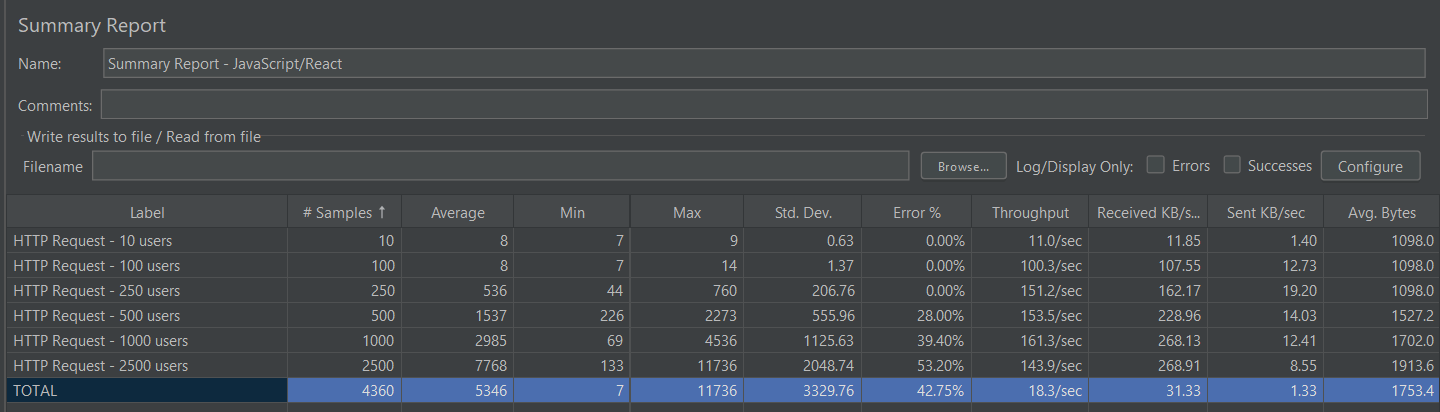
\includegraphics[width=0.8\textwidth]{Test JS load.png}
    \caption[\centering Testresultaten load test: ophalen objecten in JavaScript/React]{\label{fig:loadtest-JavaScript} Testresultaten load test: ophalen objecten in JavaScript/React}
\end{figure}


\begin{table}[h]
    \centering
    \begin{tabular}{ |p{5cm}|p{3cm}|p{3cm}|p{3cm}|}
        \hline
        \textbf{Aantal gelijktijdige \newline gebruikers} & \textbf{Gemiddelde reactietijd (ms)} & \textbf{Error \newline percentage (\%)} & \textbf{Throughput (requests/sec)}\\
        \hline
        \textbf{10}  & 8 & 0.00 & 11.0 \\
        \hline
        \textbf{100} & 8 & 0.00 & 100.3 \\
        \hline
        \textbf{250}  & 536 & 0.00 & 151.2 \\
        \hline
        \textbf{500}  & 1537 & 28.00 & 153.5 \\
        \hline                       
        \textbf{1000}  & 2985 & 39.40 & 161.3  \\
        \hline
        \textbf{2500}  & 7768 & 53.20 & 143.9 \\
        \hline
    \end{tabular}
    \caption[\centering Loadtestresultaten JavaScript/React: Kernmetrieken]{\label{tab:Testresultaten JS loadtest}Loadtestresultaten JavaScript/React: Kernmetrieken}
\end{table}


\paragraph{Mendix resultaten load testen}

\begin{figure}[H]
    \centering
    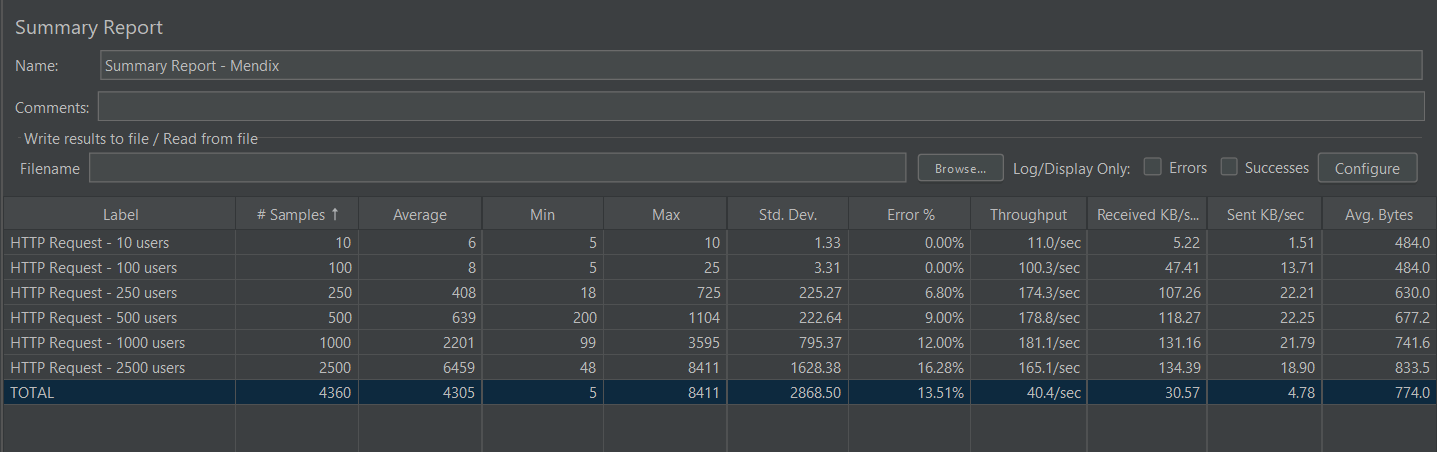
\includegraphics[width=0.8\textwidth]{Test load Mendix.png}
    \caption[\centering Testresultaten load test: ophalen objecten in Mendix]{\label{fig:loadtest-Mendix} Testresultaten load test: ophalen objecten in Mendix}
\end{figure}


\begin{table}[h]
    \centering
    \begin{tabular}{ |p{5cm}|p{3cm}|p{3cm}|p{3cm}|}
        \hline
        \textbf{Aantal gelijktijdige \newline gebruikers} & \textbf{Gemiddelde reactietijd (ms)} & \textbf{Error \newline percentage (\%)} & \textbf{Throughput (requests/sec)}\\
        \hline
        \textbf{10}  & 6 & 0.00 & 11.0 \\
        \hline
        \textbf{100} & 8 & 0.00 & 100.3 \\
        \hline
        \textbf{250}  & 408 & 6.80 & 174.3 \\
        \hline
        \textbf{500}  & 639 & 9.00 & 178.8 \\
        \hline                       
        \textbf{1000}  & 2201 & 12.00 & 181.1  \\
        \hline
        \textbf{2500}  & 6459 & 16.28 & 165.1 \\
        \hline
    \end{tabular}
    \caption[\centering Loadtestresultaten Mendix: Kernmetrieken]{\label{tab:Testresultaten Mendix loadtest}Loadtestresultaten Mendix: Kernmetrieken}
\end{table}



\paragraph{Conclusie}
Hoewel een JavaScript/React-applicatie theoretisch het potentieel heeft om Mendix te overtreffen in absolute prestaties, blijkt dit in de huidige load-testscenario’s niet het geval onder verhoogde belasting. Waar React flexibiliteit en volledige controle biedt voor optimalisatie, vereist dit ook aanzienlijke expertise en afstemming om daadwerkelijk robuust te blijven bij hoge gelijktijdige gebruikersaantallen. In de praktijk toont Mendix zich in deze tests stabieler, met name op het gebied van foutafhandeling en consistentie bij toenemende load. Dit is te danken aan de platformgebonden optimalisaties, standaardisatie en ingebouwde schaalbaarheidsmechanismen.

Beide technologieën hebben dus hun sterktes: Mendix excelleert in betrouwbaarheid en voorspelbaarheid bij grotere gebruikersvolumes, terwijl JavaScript/React – mits zorgvuldig geoptimaliseerd – de mogelijkheid biedt tot betere piekprestaties. De keuze hangt dan ook sterk af van de context en prioriteiten: snelle ontwikkeltrajecten met robuuste baseline-prestaties (Mendix) tegenover maximale flexibiliteit en performancepotentieel met meer technische investering (JavaScript/React). In de geteste scenario’s levert Mendix momenteel het meest consistente gedrag onder druk, wat voor veel toepassingen een doorslaggevend voordeel kan zijn.


\subsection{Ontwikkelsnelheid en onderhoud}

\subsubsection{Ontwikkeltijd}
De ontwikkeltijd is handmatig bijgehouden voor beide applicaties om een realistische inschatting te geven van de benodigde inspanning. Voor de JavaScript/React-applicatie bedroeg de totale ontwikkeltijd ongeveer 5 uur, waarbij tijd werd besteed aan het opzetten van de ontwikkelomgeving, het schrijven van de logica, het afhandelen van \gls{API}-calls, en het bouwen van de gebruikersinterface. Voor de Mendix-applicatie daarentegen was slechts 30 minuten nodig om een functioneel equivalent te realiseren. Deze aanzienlijke tijdwinst is te verklaren door het gebruik van vooraf gedefinieerde componenten, visuele modellering en standaardfunctionaliteit binnen het Mendix-platform. Hoewel JavaScript/React meer flexibiliteit en controle biedt, vereist het ook meer technische expertise en ontwikkelinspanning. Mendix blijkt in dit opzicht bijzonder efficiënt voor het snel realiseren van functionele prototypes of standaardapplicaties.

\subsubsection{Herbruikbaarheid / uitbreidbaarheid}
Om de aanpasbaarheid en herbruikbaarheid van componenten te evalueren, is bij beide applicaties een zoekfunctie toegevoegd. Dit biedt inzicht in hoe snel en flexibel nieuwe functionaliteit kan worden geïntegreerd. In Mendix kon de zoekfunctionaliteit in slechts 1 minuut worden geactiveerd door een bestaande zoekoptie in het component eenvoudig aan te zetten via de modeler-interface, een handeling die letterlijk neerkomt op het selecteren van een checkbox. 

\begin{figure}[H]
    \centering
    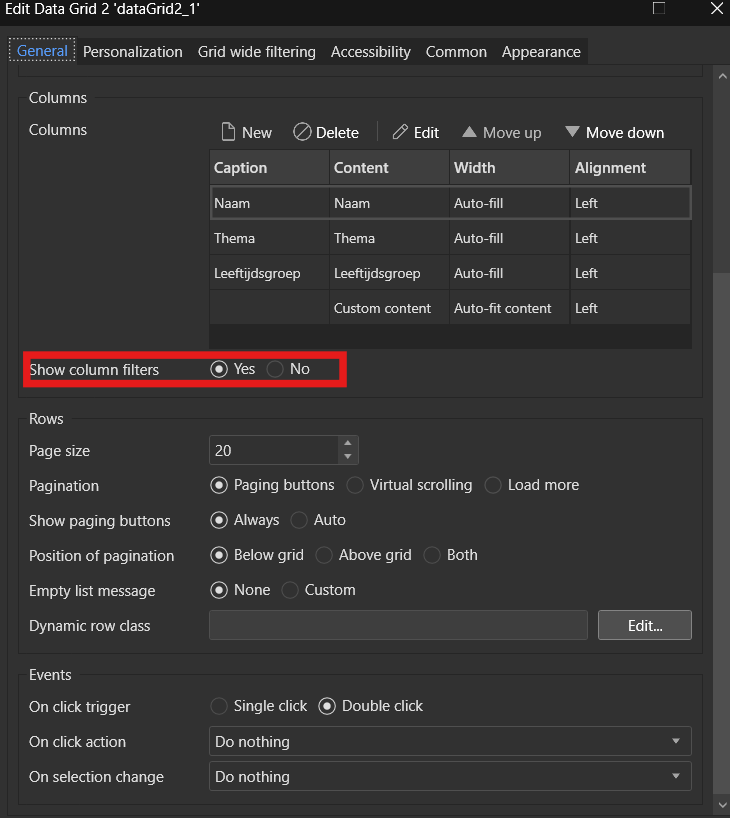
\includegraphics[width=0.5\textwidth]{show colomn filters.png}
    \caption[\centering Checkbox aanzetten filters]{\label{fig:show-colomn-filters-Mendix} Checkbox aanzetten filters}
\end{figure}


\begin{figure}[H]
    \centering
    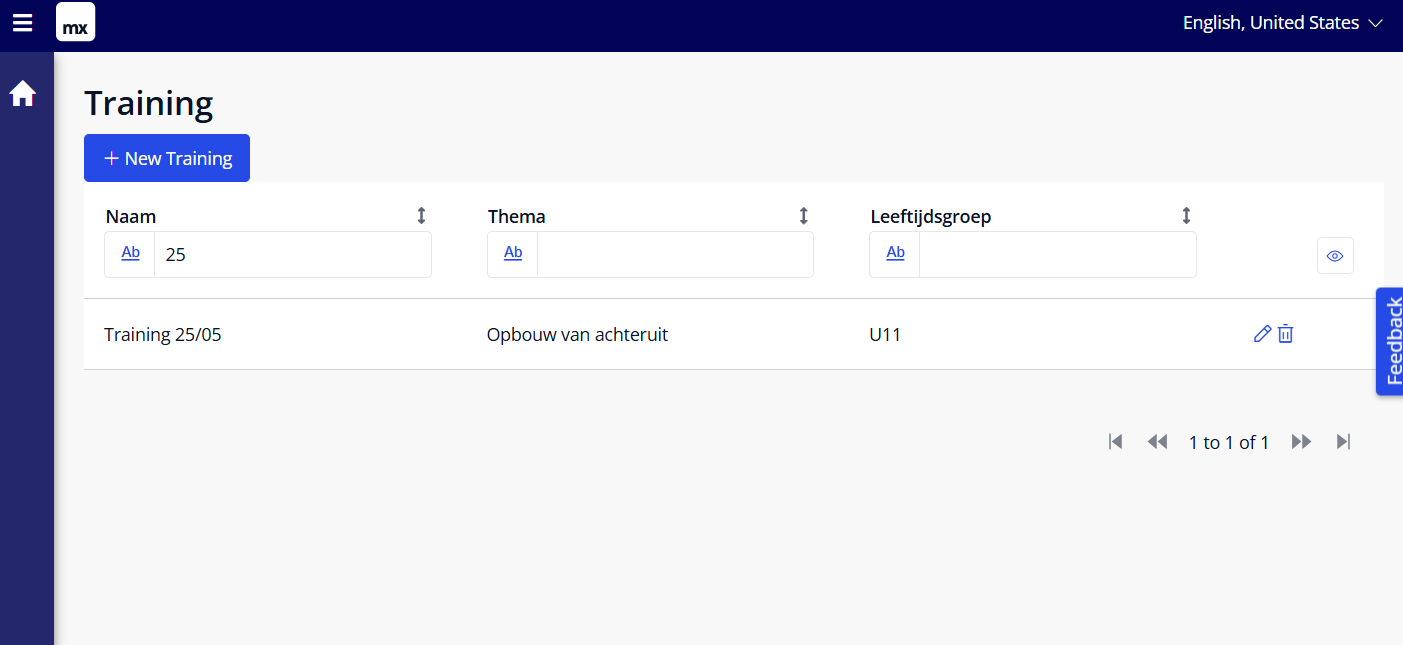
\includegraphics[width=1\textwidth]{Homepage with search Mendix.png}
    \caption[\centering Homepage with search bar]{\label{fig:homepage-with-search-Mendix} Homepage met zoekbalk Mendix}
\end{figure}



In JavaScript/React duurde het toevoegen van een vergelijkbare zoekfunctie ongeveer 15 minuten, waarbij logica handmatig moest worden geschreven, de zoekinput geïntegreerd diende te worden in de UI, en filtering op de dataset geïmplementeerd werd.

\begin{listing}[H]
        export default function TrainingsTable({ trainingen, onDelete }) {
            const [searchTerm, setSearchTerm] = useState("");
            // Filter trainingen op basis van zoekterm
            const filteredTrainingen = trainingen.filter((training) =>
            training.naam.toLowerCase().includes(searchTerm.toLowerCase())
            );
     
            if (trainingen.length === 0) {
                return <div className="alert alert-info">Nog geen trainingen.</div>;
            }
            return (
            <Box>
            {/* Zoekbalk */}
            <Input
            placeholder="Zoek op naam..."
            value={searchTerm}
            onChange={(e) => setSearchTerm(e.target.value)}
            mb={4}
            maxWidth="300px"
            />
            {/* Tabel */}
            <Table variant="striped" colorScheme="teal" size="sm">
            <Thead>
            <Tr>
            <Th>Naam</Th>
            <Th>Thema</Th>
            <Th>Leeftijdsgroep</Th>
            <Th></Th>
            </Tr>
            </Thead>
            <Tbody>
            {filteredTrainingen.length > 0 ? (
                filteredTrainingen.map((training) => (
                <Training key={training.id} onDelete={onDelete} {...training} />
                ))
                )}
            </Tbody>
            </Table>
            </Box>
            );
        }
    \caption{Trainingstabel met zoekfunctie op naam}
    \label{lst:pipeline-clone}
\end{listing}

\begin{figure}[H]
    \centering
    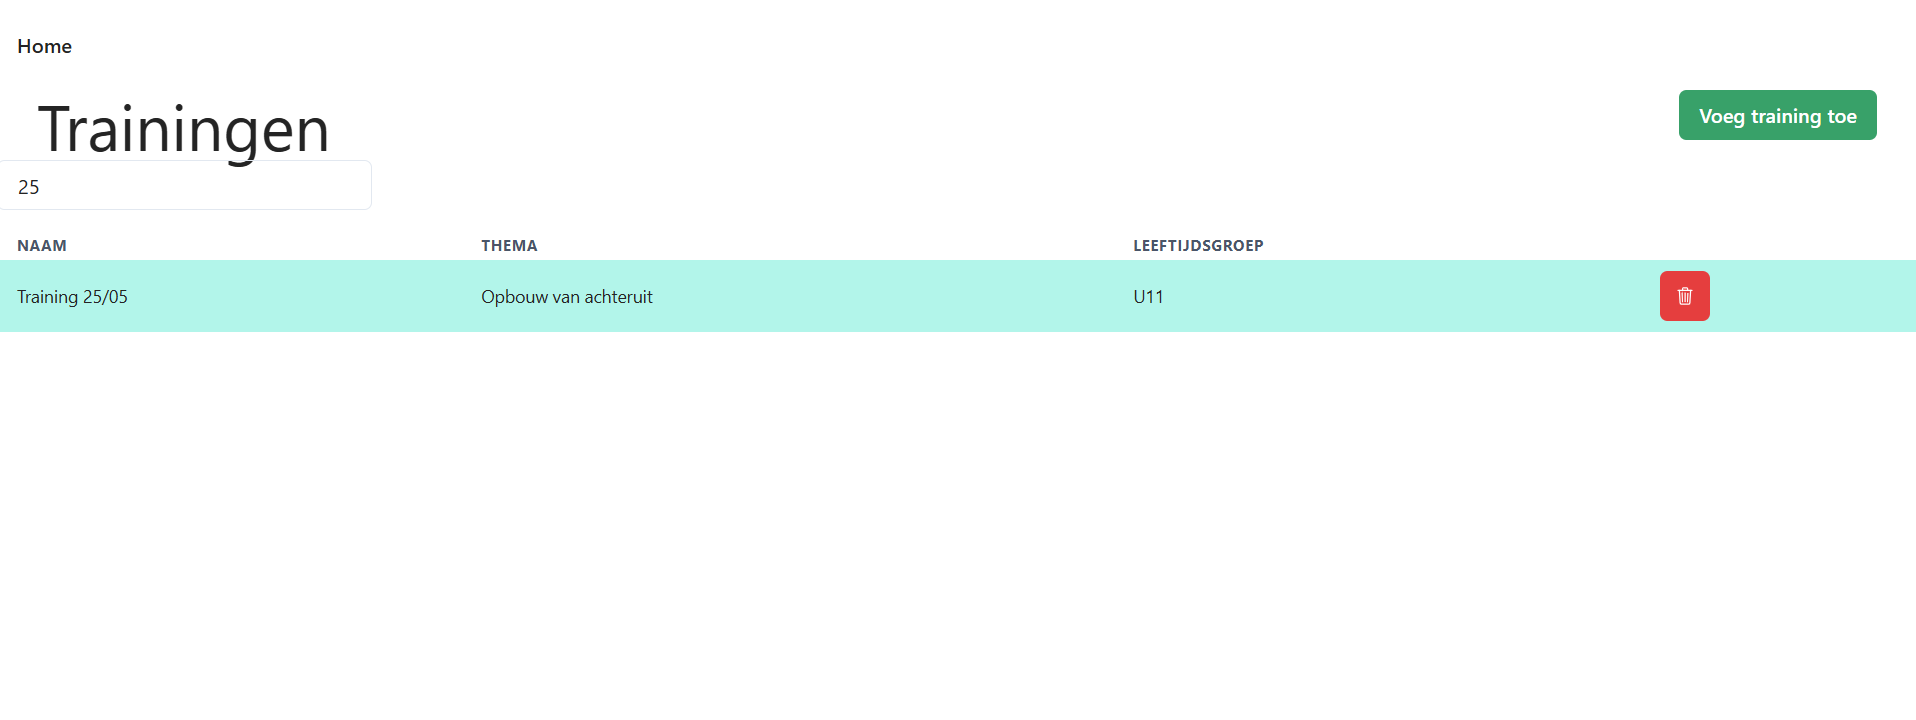
\includegraphics[width=1\textwidth]{Homepage with search JS.png}
    \caption[\centering Homepage with search bar JavaScript/React]{\label{fig:homepage-with-search-JS} Homepage met zoekbalk JavaScript/React}
\end{figure}


 Hoewel de implementatie in beide gevallen vlot verliep, toont dit voorbeeld aan dat Mendix dankzij herbruikbare en vooraf geconfigureerde componenten bijzonder efficiënt is bij het uitbreiden van functionaliteit, terwijl JavaScript/React meer flexibiliteit biedt maar ook meer ontwikkelwerk vraagt.


\subsection{Integratiemogelijkheden}

Zowel Mendix als JavaScript/React bieden uitgebreide mogelijkheden om te integreren met externe systemen, maar de manier waarop deze integraties tot stand komen verschilt aanzienlijk vanwege hun aard: Mendix als low-code platform en JavaScript/React als code-first benadering.

\subsubsection{Mendix}

Mendix is ontworpen om eenvoudig te koppelen met zowel moderne als legacy systemen, met standaard ondersteuning voor verschillende integratietechnieken:
\begin{itemize}
    \item \textbf{REST \gls{API}'s}: volledige ondersteuning voor het bouwen en consumeren van RESTful APIs. Integraties zoals met Salesforce of SAP zijn vlot op te zetten via visuele flows.
    \item \textbf{SOAP Webservices}: ondersteuning voor oudere protocollen blijft behouden, wat belangrijk is voor bedrijven met legacy infrastructuren.
    \item \textbf{GraphQL}: niet native ondersteund, maar via extensies of community-modules kunnen GraphQL-endpoints alsnog worden aangesproken.
    \item \textbf{OData Services}: Mendix biedt OData-integraties voor onder meer BI-tools zoals Power BI.
    \item \textbf{JDBC-databaseconnecties}: directe verbinding met relationele databases zoals SQL Server, MySQL, PostgreSQL en Oracle.
\end{itemize}

Daarnaast is er toegang tot Mendix Connect en de Mendix Marketplace, waar herbruikbare connectors beschikbaar zijn voor populaire systemen zoals SAP, Salesforce, Kafka en meer. Dit maakt het voor ontwikkelaars mogelijk om snel integraties op te zetten zonder complexe code.

\subsubsection{JavaScript/React}

JavaScript/React biedt in essentie volledige vrijheid voor integratie, maar dit betekent ook dat ontwikkelaars zelf verantwoordelijk zijn voor de implementatie van alle benodigde logica en security rond die integraties:
\begin{itemize}
    \item \textbf{REST en GraphQL}: beide worden uitstekend ondersteund via moderne bibliotheken zoals Axios, Fetch API, Apollo Client of Relay.
    \item \textbf{WebSocket en realtime communicatie}: makkelijk op te zetten met bibliotheken zoals Socket.IO.
    \item \textbf{SOAP}: mogelijk, maar vereist aparte libraries (zoals soap in Node.js), aangezien SOAP minder gangbaar is in moderne JavaScript-ecosystemen.
    \item \textbf{Directe databaseverbindingen}: in een typische React frontend niet van toepassing, maar in combinatie met een Node.js backend kunnen via ORM's (zoals Sequelize, Prisma) databases als MySQL, PostgreSQL of MongoDB worden aangesproken.
\end{itemize}

JavaScript/React biedt maximale controle, flexibiliteit en toegang tot een breed scala aan open-source libraries en SDK’s. Wel vraagt het opzetten van integraties meer technische kennis en aandacht voor zaken als foutafhandeling, authenticatie (OAuth, JWT) en datastructurering.

\subsubsection{Vergelijking}

\begin{table}[H]
    \centering
    \begin{tabular}{ |p{3cm}|p{5.5cm}|p{5.5cm}|}
        \hline
        \textbf{Aspect} & \textbf{Mendix} & \textbf{JavaScript/React}\\
        \hline
        \textbf{Complexiteit}  & Laag, via visuele modelering en kant-en-klare connectors & Hoog, handmatig implementeren via code  \\
        \hline
        \textbf{Ondersteunde protocollen} & REST, SOAP, OData, JDBC, GraphQL (indirect) & REST, GraphQL, WebSockets, SOAP (met lib) \\
        \hline
        \textbf{Herbruikbare integraties}  & Beschikbaar via Mendix Marketplace & 	Zelf te beheren of via externe NPM packages \\
        \hline
        \textbf{Flexibiliteit}  & 	Beperkt tot wat het platform ondersteunt & Zeer hoog, volledige controle over gedrag \\
        \hline                       
        \textbf{Snelheid van integratie}  & 	Zeer snel (minuten) met visuele ondersteuning & Langzamer (uren), afhankelijk van de setup \\
        \hline
    \end{tabular}
    \caption[\centering Integratiemogelijkheden]{\label{tab:integratiemogelijkheden}Integratiemogelijkheden}
\end{table}
In essentie is Mendix zeer geschikt wanneer snelheid, standaardisatie en visuele eenvoud voorop staan. JavaScript/React is de juiste keuze wanneer maximale flexibiliteit, diepgaande aanpassing en custom integraties vereist zijn — mits de nodige technische expertise aanwezig is.


\subsection{Aanpasbaarheid en uitbreidbaarheid}

Het Mendix-platform combineert de snelheid van low-code ontwikkeling met voldoende flexibiliteit voor geavanceerde uitbreidingen. Standaard biedt Mendix een brede waaier aan voorgeprogrammeerde blokken en componenten, zoals widgets, datakoppelingen, validatieacties en gebruikersinterface-elementen, die eenvoudig via drag-and-drop in de applicatie kunnen worden geïntegreerd. Deze componenten versnellen het ontwikkelproces aanzienlijk en vereisen minimale configuratie.

Toch blijft het platform niet beperkt tot wat standaard beschikbaar is. Voor situaties waarin maatwerk vereist is, biedt Mendix meerdere uitbreidingsmogelijkheden:
\begin{itemize}
    \item \textbf{Java-acties}: voor het uitvoeren van complexe server-side logica kunnen aangepaste Java-methoden worden ingebouwd.
    \item \textbf{Pluggable widgets}: ontwikkelaars kunnen hun eigen UI-componenten maken in JavaScript of React, die vervolgens naadloos integreren met het Mendix-model.
    \item \textbf{Mendix Model SDK}: hiermee kunnen ontwikkelaars programmatic wijzigingen aanbrengen in het domeinmodel of app-logica, bijvoorbeeld voor codegeneratie of CI/CD-integratie.
    \item \textbf{Extensibility \gls{API}}: maakt het mogelijk om Studio Pro zelf uit te breiden met nieuwe functionaliteit, wat handig is voor grotere ontwikkelteams of platformontwikkeling.
\end{itemize}

In vergelijking met JavaScript/React biedt Mendix een meer gestandaardiseerde aanpak, waarbij veelgebruikte patronen al zijn voorgedefinieerd. Dit maakt het zeer efficiënt voor snelle ontwikkeling en eenvoudige aanpassingen. JavaScript/React daarentegen biedt volledige vrijheid en maatwerk vanaf nul, maar vereist meer handmatige inspanning en technische kennis voor uitbreidbaarheid.

Mendix positioneert zich daarmee als een platform dat zowel toegankelijk is voor snelle ontwikkeling via visuele bouwblokken, als krachtig genoeg om uit te breiden wanneer standaardcomponenten niet volstaan, zonder de ontwikkelaar volledig vast te zetten binnen het framework.


\subsection{Beveiliging en compliance}

Beveiliging en compliance zijn cruciale aspecten bij de ontwikkeling van moderne toepassingen, en zowel Mendix als JavaScript/React bieden hier oplossingen voor wel  op verschillende manieren.

\subsubsection{Mendix}

Mendix hecht veel waarde aan beveiliging en biedt een breed scala aan ingebouwde beveiligingsmechanismen. Standaard voorziet het platform in:
\begin{itemize}
    \item \textbf{Rollen- en toegangsbeheer op applicatie- en entiteitniveau}, configureerbaar via de modeler.
    \item \textbf{Gegevensversleuteling} zowel in rust als tijdens transport.
    \item \textbf{Authenticatie-integratie} met SSO, OAuth 2.0, SAML en Active Directory.
    \item \textbf{Automatische beveiligingsupdates} en naleving van standaarden zoals ISO 27001, SOC 2 en GDPR.
\end{itemize}

Doordat veel beveiligingsmaatregelen standaard in het platform zitten, hoeven ontwikkelaars zich minder zorgen te maken over implementatiedetails. Daarnaast ondersteunt Mendix opslag in beheerde of eigen SQL-databases (zoals PostgreSQL, MS SQL of Oracle), wat organisaties flexibiliteit biedt in gegevensbeheer en compliance.

\subsubsection{JavaScript/React}

In een JavaScript/React-omgeving ligt de verantwoordelijkheid voor beveiliging volledig bij het ontwikkelingsteam. React zelf biedt geen beveiligingsfunctionaliteit; beveiliging moet worden geïmplementeerd via aanvullende tools en best practices:
\begin{itemize}
    \item \textbf{Toegangscontrole en authenticatie} worden vaak geregeld via third-party services (zoals Auth0, Firebase Auth) of via backend-implementaties (JWT, OAuth).
    \item \textbf{Encryptie en veilige opslag} moeten handmatig worden geconfigureerd op server- en transportniveau (bv. HTTPS, TLS, encryptie van gevoelige data in databases).
    \item \textbf{Veiligheidsrisico’s zoals XSS en CSRF} moeten proactief worden gemitigeerd via frameworks of headers (CSP, SameSite cookies, sanitization).
    \item \textbf{Compliance} met regelgeving (zoals GDPR) vereist eigen implementatie van dataverwerking, audit logging en toestemmingsbeheer.
\end{itemize}

Hoewel React dus maximale controle biedt, vraagt het ook een aanzienlijke investering in kennis en tooling om een vergelijkbaar beveiligingsniveau als bij Mendix te bereiken.


\subsubsection{Vergelijking}

Mendix biedt een zeer veilig ecosysteem met veel standaardmaatregelen die de ontwikkelaar ontlasten. Voor organisaties met strikte compliance-eisen of beperkte beveiligingsexpertise is dit een groot voordeel. JavaScript/React daarentegen biedt volledige vrijheid en controle, maar vereist een zorgvuldige en goed onderbouwde aanpak om dezelfde mate van beveiliging en compliance te realiseren.


\subsection{Samenvattende conclusie praktisch onderzoek}
Uit het praktisch onderzoek blijkt dat zowel Mendix als JavaScript/React sterke troeven bieden voor de ontwikkeling van moderne webapplicaties, maar dat hun inzetbaarheid sterk afhankelijk is van de context en vereisten van het project.

Qua integratiemogelijkheden toont Mendix zich als een krachtig low-code platform met standaard ondersteuning voor veelgebruikte protocollen zoals REST, SOAP en OData. De beschikbaarheid van kant-en-klare connectors via de Mendix Marketplace zorgt voor snelle, visuele integratie met externe systemen. JavaScript/React daarentegen biedt maximale flexibiliteit en controle bij het integreren met externe services, maar vereist meer technische expertise en handmatige implementatie.

Op vlak van aanpasbaarheid en uitbreidbaarheid scoort Mendix hoog met zijn pluggable widgets, Java-acties en Model SDK, wat toelaat om standaardcomponenten uit te breiden wanneer nodig. Toch blijft JavaScript/React onovertroffen in maatwerk en volledige controle over zowel front- als backendlogica, zij het met een hogere ontwikkelkost.

Wat beveiliging en compliance betreft, biedt Mendix een veilig ecosysteem met veel ingebouwde maatregelen en certificeringen, wat het platform bijzonder geschikt maakt voor organisaties met hoge compliance-eisen of beperkte beveiligingsexpertise. JavaScript/React vereist daarentegen een meer proactieve aanpak van het ontwikkelingsteam om dezelfde beveiligingsstandaarden te behalen.

Samengevat is Mendix ideaal voor projecten waarbij snelheid, standaardisatie en visuele ontwikkeling centraal staan, terwijl JavaScript/React de voorkeur geniet in situaties waar volledige controle, flexibiliteit en diepgaande technische aanpassing vereist zijn. De keuze tussen beide technologieën is dus geen kwestie van beter of slechter, maar eerder van passend bij het juiste type project en ontwikkelteam.


\section{Reflectie op eigen ervaringen}
Op basis van mijn ervaring kan ik bevestigen dat low-code, zoals Mendix, bijzonder krachtig is voor het snel opzetten van generieke applicaties met standaardfunctionaliteiten. Het stelt je in staat om in korte tijd werkende oplossingen te bouwen, wat vooral in iteratieve of proof-of-concept contexten een grote meerwaarde biedt. Tegelijk merk ik dat zodra een project meer ‘custom’ noden heeft – zoals complexe bedrijfslogica of verfijnde integraties – de grenzen van het platform sneller voelbaar worden. In die gevallen is het een duidelijke troef om een high-code achtergrond te hebben: je begrijpt beter wat er onder de motorkap gebeurt, kunt gerichter zoeken naar workarounds en neemt bewuster beslissingen over de architectuur van je oplossing. Bovendien zie ik dat een traditionele programmeerachtergrond ook de leesbaarheid en structuur van je low-code logica ten goede komt. Je denkt in patronen, zorgt voor herbruikbaarheid en hanteert best practices die niet vanzelfsprekend zijn in een puur visuele ontwikkelomgeving.

\subsection{Reflectie op ervaringen van experts}
Er zijn ook enkele ontwikkelaars met een klassieke high-code achtergrond die inmiddels volledig actief zijn binnen low-code projecten, met name op het Mendix-platform. Ik sprak met hen over hun ervaringen en vatte hun bevindingen samen. 
Ze benadrukken dat low-code bijzonder krachtig is voor het snel ontwikkelen van generieke applicaties met standaardfunctionaliteiten. Dit maakt het ideaal voor situaties waarin snelheid en iteratieve ontwikkeling belangrijk zijn. Daarnaast wordt low-code vaak gepositioneerd als een brug tussen IT en business, doordat ook gebruikers zonder programmeerervaring relatief snel aan de slag kunnen. In de praktijk leidde dit er echter soms toe dat businessgebruikers eigen applicaties opstartten die later door ervaren ontwikkelaars moesten worden overgenomen. Deze overdracht bleek niet altijd evident: de onderliggende logica bleek vaak moeilijk leesbaar en voldeed zelden aan gangbare ontwikkelstandaarden of best practices, wat extra werk met zich meebracht om de applicatie te stabiliseren en verder te ontwikkelen.

Wat betreft de ontwikkelervaring binnen Mendix, werd er gemengd gereageerd op de version control-functionaliteit. Hoewel het systeem in principe krachtig is en goed integreert met teamwerk, kunnen foutmeldingen en merge-conflicten soms moeilijk te doorgronden zijn. Wanneer alles echter correct functioneert, biedt het versiebeheer een betrouwbare en efficiënte manier van samenwerken. De integratie van agile werkmethodieken binnen het Mendix-platform werd unaniem positief beoordeeld: user stories, sprints en voortgang kunnen rechtstreeks via de projectpagina opgevolgd en beheerd worden, wat de samenwerking tussen ontwikkelaars en stakeholders vergemakkelijkt.

Ook het gebruik van herbruikbare modules uit de Mendix Marketplace werd als een groot voordeel genoemd. Het toevoegen van bestaande componenten versnelt de ontwikkeling aanzienlijk en voorkomt dat het wiel telkens opnieuw moet worden uitgevonden. Tegelijk wordt opgemerkt dat een groot aantal van deze modules weinig tot geen documentatie bevat, waardoor het tijd kost om hun werking te doorgronden of aan te passen aan specifieke projectbehoeften. 

Over het geheel genomen beschouwen deze ontwikkelaars Mendix als een toegankelijke en efficiënte ontwikkelomgeving, die eenvoudig aanvoelt in de basis, maar bij complexere noden ook de nodige technische diepgang vereist. Hun ervaring met high-code vormt daarbij een duidelijke meerwaarde: het helpt hen om concepten sneller te begrijpen, kwalitatieve oplossingen te bouwen en de leesbaarheid en onderhoudbaarheid van hun low-code toepassingen te verbeteren.

\section{Evaluatie van Mendix-uitbreidingen}
Op basis van gesprekken met ervaren ontwikkelaars die dagelijks met Mendix werken, blijkt dat het gebruik van standaard Marketplace-modules doorgaans als efficiënt en tijdbesparend wordt ervaren, vooral bij generieke functionaliteiten. Deze modules kunnen snel geïntegreerd worden, wat de implementatietijd aanzienlijk verkort. Toch werd ook opgemerkt dat veel van deze modules onvoldoende of zelfs geheel geen documentatie bevatten. Dit gebrek aan transparantie leidt tot vertragingen tijdens implementatie en beperkt de flexibiliteit wanneer aanpassingen nodig zijn. In zulke gevallen biedt custom ontwikkeling vaak meer controle en beter afgestemde oplossingen, hoewel dit uiteraard gepaard gaat met een langere ontwikkeltijd en hogere initiële kosten.

Java-uitbreidingen binnen Mendix worden door ontwikkelaars met een high-code achtergrond beschouwd als waardevolle tools om de beperkingen van het platform te omzeilen, bijvoorbeeld bij complexe logica of integraties met externe systemen. Deze uitbreidingen verhogen echter ook de technische complexiteit van het project en kunnen de onderhoudbaarheid op lange termijn negatief beïnvloeden, zeker wanneer ze niet goed gedocumenteerd zijn of slechts door een beperkte groep binnen het team begrepen worden.

Wat betreft de kosten-batenverhouding, geven ontwikkelaars aan dat low-code in combinatie met herbruikbare modules initieel voordeliger is in zowel ontwikkeling als beheer. Naarmate de applicatie complexer wordt en meer ‘maatwerk’ vereist, verschuift dit evenwicht echter, en kunnen custom uitbreidingen of Java-integraties duurder uitvallen, zowel in termen van ontwikkeluren als bij latere aanpassingen of onderhoud.

Tot slot werd ook het integreren van externe systemen als een uitdaging benoemd. Hoewel Mendix hier voldoende ondersteuning voor biedt, vergt het combineren van low-code met externe services een goed begrip van beide kanten. Een technische achtergrond blijkt in die context bijzonder waardevol, zowel voor het begrijpen van de externe API’s als voor het bouwen van robuuste, onderhoudbare koppelingen binnen het platform. Al met al tonen deze bevindingen aan dat een doordachte strategie, met oog voor schaalbaarheid en onderhoud, essentieel is bij het uitbreiden van Mendix-toepassingen.

\section{Ontwikkeling beslissingskader}

\subsection{Cijfermatige evaluatiematrix}
Voor een snelle vergelijking tussen Mendix en traditionele ontwikkeling is in Tabel~\ref{tab:beslissingsmatrix} een scorematrix opgenomen. Per dimensie is een score van 1 tot 5 toegekend, waarbij 5 duidt op een sterke geschiktheid van de technologie in die context. Deze matrix ondersteunt de eerste oriëntatie in het besluitvormingsproces.

\begin{table}[H]
    \centering
    \begin{tabular}{|p{3cm}|p{5cm}|p{2cm}|p{4cm}|}
        \hline
        \textbf{Dimensie} & \textbf{Vraag} & \textbf{Score (1–5)} & \textbf{Toelichting} \\
        \hline
        \textbf{Tijd \& Scope} & Moet er binnen enkele \newline weken een MVP live zijn? & & 1 = Ja, 5 = Nee \\
        \cline{2-4}
         & Is het project iteratief/ veranderlijk (agile, MVP-gedreven)? & & 1 = Sterk veranderlijk, 5 = Vast ontwerp \\
        \hline
        \textbf{Technische \newline Vereisten} & Is de businesslogica \newline complex of sterk veranderlijk? & & 1 = Simpel, 5 = \newline Complex/custom \newline algoritmes \\
        \cline{2-4}
         & Zijn real-time functionaliteiten vereist (sockets, streaming)? & & 1 = Nee, 5 = Ja \\
        \hline
        \textbf{Teamcapaciteit} & Is er voldoende high-code ontwikkelcapaciteit aanwezig? & & 1 = Beperkt, 5 = Ruim beschikbaar \\
        \cline{2-4}
         & Beschikt het team over mensen met domeinkennis die actief kunnen bijdragen aan de ontwikkeling? & &1 = Niet aanwezig, \newline 5 = Actief betrokken \\
        \hline
        \textbf{Integratiebe- hoefte} & Betreft het veel standaard systemen (SAP, \newline Salesforce)? & & 1 = Ja, 5 = Nee \\
        \cline{2-4}
         & Gaat het om non-standaard of complexe API-integraties? & & 1 = Nee, 5 = Ja \\
        \hline
        \textbf{UX/Design} & Moet de UI sterk afwijken van \newline standaardcomponenten? & & 1 = Nee, 5 = Ja \\
        \cline{2-4}
         & Is er nauwe \newline samenwerking nodig met UX-designers of brandingteams? & & 1 = Beperkt, 5 = \newline Intensief \\
        \hline
        \textbf{Beveiliging \& Compliance} & Zijn er strikte eisen (GDPR, ISO, interne audits)? & & 1 = Ja, 5 = Nee \\
        \cline{2-4}
         & Wordt gevoelige of gereguleerde data verwerkt? & & 1 = Ja, 5 = Nee \\
        \hline
    \end{tabular}
    \caption{Beslissingsmatrix}
    \label{tab:beslissingsmatrix}
\end{table}

\subsubsection{Interpretatie van de score}
De totaalscore op basis van de beoordelingsmatrix uit Sectie 2 biedt richting bij de keuze van ontwikkelmethode:

\begin{itemize}
    \item \textbf{12–27 punten: Mendix aanbevolen} \\
    Geschikt voor projecten die vragen om snelheid, visueel modelleren, standaardisatie en minder technische complexiteit.
    
    \item \textbf{28–44 punten: Hybride oplossing overwegen} \\
    Combineer Mendix met traditionele ontwikkeling, bijvoorbeeld Mendix voor workflows en beheerfuncties, en traditionele technologieën voor UI of complexe businesslogica.
    
    \item \textbf{45–60 punten: High-code ontwikkeling aanbevolen} \\
    Vereist maximale flexibiliteit, diepgaande technische implementaties of specifieke designvereisten die moeilijk in low-code te realiseren zijn.
\end{itemize}

\paragraph{Let op:} Bij een hybride of twijfelgeval speelt het teamvertrouwen een belangrijke rol. Als een team meer ervaring of vertrouwen heeft in één van beide technologieën, verdient het de voorkeur om die richting te volgen, mits dit past binnen de technische kaders van het project.

De matrix fungeert als sneltoets, maar dient aangevuld te worden met projectcontext en nuance. Hiervoor zijn verdiepende beoordelingsvragen opgenomen in de volgende paragraaf.

\subsection{Verdiepende beoordelingsvragen per dimensie}
Naast de scorematrix kunnen onderstaande vragen projectteams helpen om de keuze kwalitatief verder te onderbouwen. Deze vragen zijn bedoeld voor dialoog en analyse tijdens de initiële architectuursessies.

\paragraph{Tijd \& Scope}
\begin{itemize}
    \item Hoe kritisch is het dat er binnen enkele weken een MVP beschikbaar is?
    \item Wordt het project agile opgezet, met ruimte voor iteratie en bijsturing?
\end{itemize}

\paragraph{Technische vereisten}
\begin{itemize}
    \item Hoe complex en veranderlijk is de businesslogica?
    \item Zijn real-time updates, complexe berekeningen of algoritmes vereist?
\end{itemize}

\paragraph{Teamcapaciteit}
\begin{itemize}
    \item Zijn er voldoende ervaren high-code ontwikkelaars (JavaScript, backend) beschikbaar?
    \item Zijn er medewerkers die met low-code tools overweg kunnen (bijv. functioneel beheerders)?
\end{itemize}

\paragraph{Integratiebehoefte}
\begin{itemize}
    \item Wordt integratie gevraagd met veelvoorkomende systemen (zoals SAP, Salesforce)?
    \item Zijn er non-standaard koppelingen of legacy-systemen zonder moderne APIs?
\end{itemize}

\paragraph{UX / Design}
\begin{itemize}
    \item Is een pixel-perfect design vereist dat afwijkt van standaardcomponenten?
    \item Moet intensief worden samengewerkt met UX-designers of brandingteams?
\end{itemize}

\paragraph{Beveiliging \& Compliance}
\begin{itemize}
    \item Zijn er compliance-eisen zoals GDPR, ISO27001 of interne audits?
    \item Wordt er gewerkt met gevoelige, persoonsgebonden of gereguleerde data?
\end{itemize}


\subsection{Richtlijnen voor hybride projecten}
Bij veel projecten is een zuivere keuze tussen Mendix en traditionele ontwikkeling niet zwart-wit. In complexe omgevingen is een \textit{hybride benadering} vaak het meest geschikt: low-code wordt ingezet waar snelheid en standaardisatie gewenst zijn, terwijl traditionele high-code wordt benut voor maatwerk en technische diepgang.

Een succesvolle hybride opzet vereist een duidelijke architectuur en samenwerking tussen beide ontwikkelvormen. Belangrijke aandachtspunten hierbij zijn:

\begin{itemize}
    \item \textbf{Functionele splitsing:} Bepaal vooraf welke onderdelen zich lenen voor low-code, en welke beter passen binnen traditionele ontwikkeling. Denk in termen van componenten, niet van hele applicaties.
    
    \item \textbf{Afstemming via API’s:} Zorg voor goed gedefinieerde interfaces en communicatieprotocollen tussen Mendix- en high-codecomponenten. Gebruik hierbij gestandaardiseerde formats zoals REST, JSON en OpenAPI.
    
    \item \textbf{Gedeeld ontwikkelproces:} Gebruik één gezamenlijke backlog, gezamenlijke sprintplanning en continue afstemming tussen beide ontwikkelteams. Dit voorkomt dat de low-code en high-code delen van elkaar vervreemden.
    
    \item \textbf{Kwaliteitsbewaking:} Pas testautomatisering, code reviews en monitoring toe op zowel Mendix als traditionele code. Behandel low-codecomponenten niet als ‘bijzaak’, maar als volwaardige onderdelen van het systeem.
    
    \item \textbf{Teamvertrouwen en ervaring:} Bij twijfel of overlap, geef voorkeur aan de technologie waar het team het meeste vertrouwen of ervaring mee heeft—mits dit binnen de technische vereisten past. Stabiliteit en beheersbaarheid gaan boven dogmatische keuzes.
\end{itemize}

Deze hybride aanpak biedt organisaties het beste van beide werelden: de snelheid en toegankelijkheid van Mendix, gecombineerd met de kracht en controle van traditionele ontwikkeling. Voorwaarde is wel dat er duidelijke kaders en technische governance worden ingericht om deze samenwerking structureel in goede banen te leiden.



